\subsection{Instruction Decode stage} 
\label{section:stage_id}

The instruction decode stage is responsible for producing the correct control signals and reading and writing the register file. As a consequence of the pipelined design the stage also contains logic for masking the errors that occurs.

\begin{figure}[h]
        \centering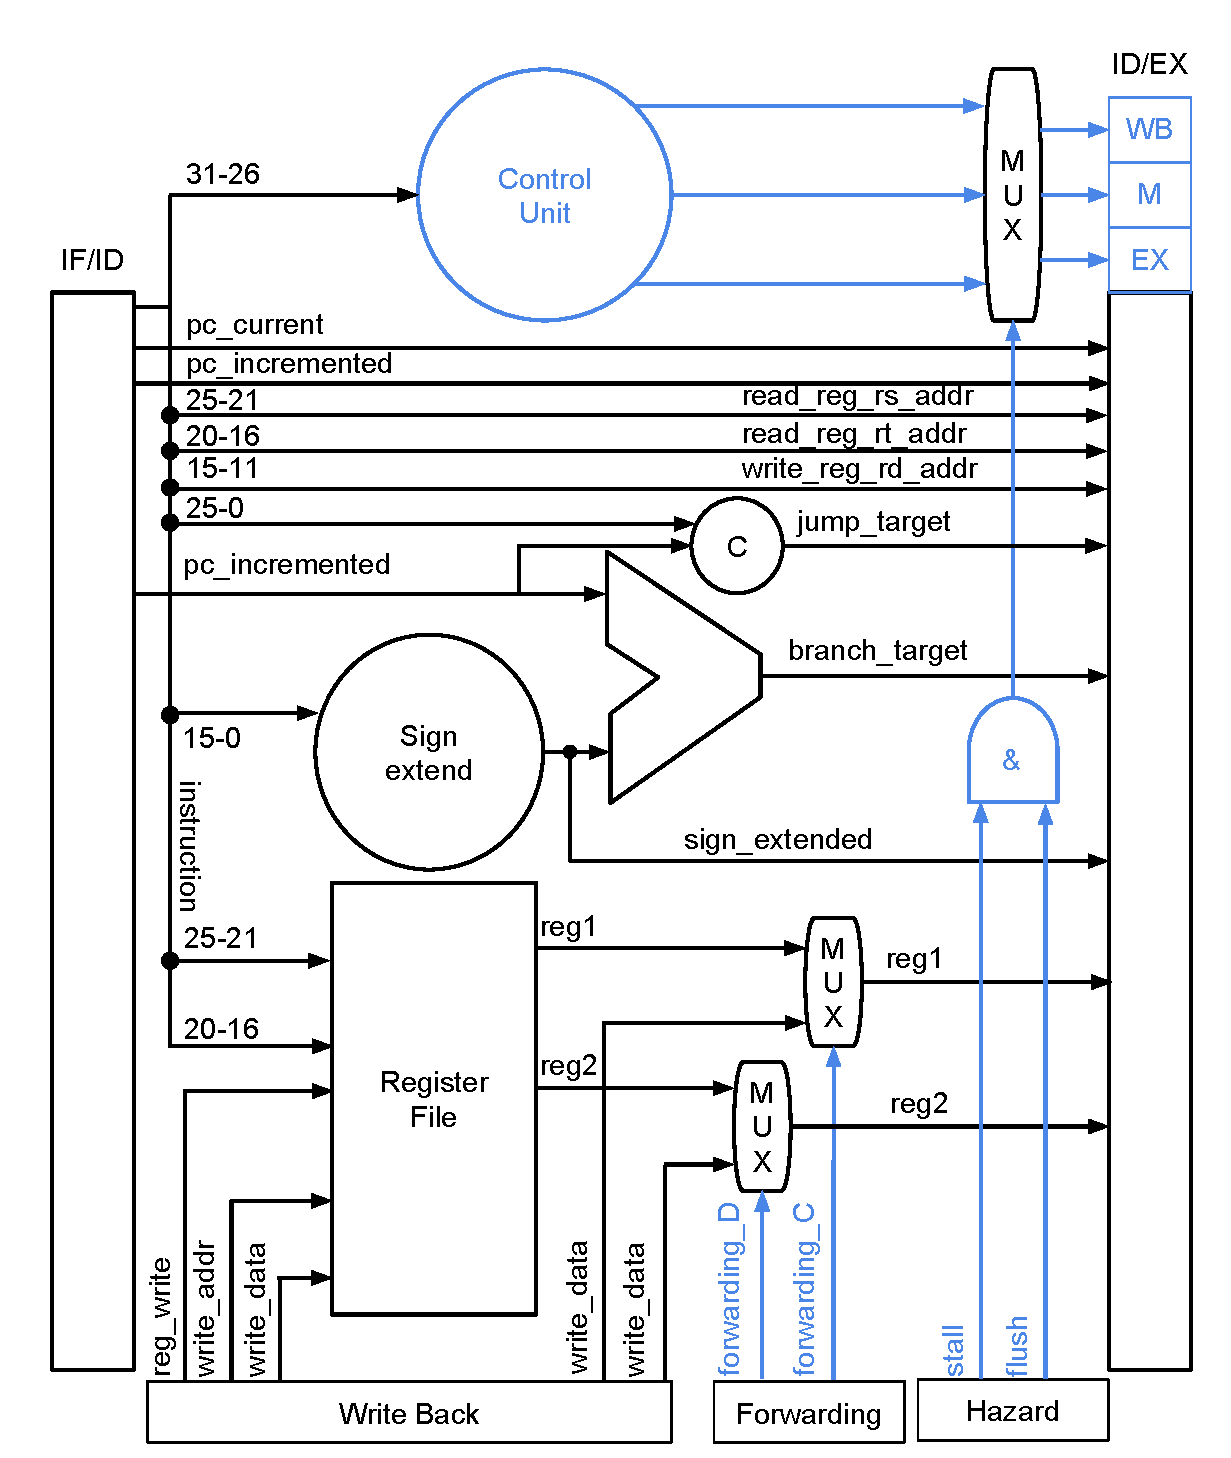
\includegraphics[scale=0.5]{figures/stage_id}
        \caption{The stage\_id architecture}
         \label{fig:stage_id}
\end{figure}
\FloatBarrier

On the top of figure \ref{fig:stage_id} the first 8 bits of the instruction are passed to the control unit. The unit produces the same control singals as in the multicycle design \cite{multicycle}, but grouped in three groups depending on the stage the signal manipulates. Before the control signals are sent to the next stage they go through a multiplexer used for creating no-ops. These no-ops are used when the stall and flush signals are asserted from the hazard detection unit. Below the control unit, the pc and pc incremented signals are passed to the next stage. These are used by the branch predictor to predict and correct branching. The next three lines forwards the rs, rt and rd address portions from the instructions. They are propagated through to the write back stage and returns to the id stage in the bottom left corner. The names here are poorly chosen as the \emph{read\_reg\_rt\_addr} is used as the write address in all I-type instructions. The middle section containing the C (concat), Sign Extend and Add units computes jump and branch targets while forwarding the result of the sign extension. The jump target is used at the processor level to perform jumping, the branch target is used in the execute stage along with the sign extended value. The bottom half of the figure contains the register file and two multiplexers which handles forwarding results from the write back stage to the execute stage. Here the design differes from that of the text book \cite{curriculum}. In the book, the values written to the register in the write back stage propagates through the register file and to the execute input register in one cycle. As the register file is clocked this is not the case with the processor described in this report. Two additional forwarding paths are added, analogous to those in the execute stage. They are used when an instruction in the id stage reads from the same register as an instruction in the write back stage is writing to.

\subsubsection{Control Unit}
The control unit for the pipelined processor is highly simplified from the one implemented in the multicycle design \cite{multicycle}. In the multicycle this unit was implemented as a state machine, while its pipeline equivalent is a combinatorical circuit. The output, shown in table \ref{table:control_signals}, is identical to the output in the execute stage from the multicycle processor.

\begin{table}[h]
	\begin{tabular}{l|l|l|l|l|l|l|l|l|l|l|l}
    \swtext{Opcode} &
    \swtext{jump} & 
    \swtext{reg\_dst} & 
    \swtext{branch}  &
    \swtext{alu\_src} &
    \swtext{alu\_op} &
    \swtext{mem\_write} &
    \swtext{mem\_read} &
    \swtext{mem\_to\_reg} &
    \swtext{reg\_write}   \\
 
    \hline
    & \multicolumn{5}{|l|}{ctrl\_ex} & \multicolumn{2}{|l|}{ctrl\_m} & \multicolumn{2}{|l|}{ctrl\_wb} \\
    \hline
    000000 (ALU)    & 0 & 1 & 0 & 0 & FUNC        & 1 & 0 & 0 & 0 \\ 
    100011 (LW)     & 0 & 0 & 0 & 1 & LOAD\_STORE & 1 & 1 & 0 & 1 \\
    101011 (SW)     & 0 & 0 & 0 & 1 & LOAD\_STORE & 0 & 0 & 1 & 1 \\  
    001111 (LUI)    & 0 & 0 & 0 & 1 & LDI         & 1 & 0 & 0 & 1 \\
    000100 (BEQ)    & 0 & 1 & 1 & 0 & BRANCH      & 0 & 0 & 0 & 0 \\  
    000010 (J)      & 1 & 1 & 0 & 0 & BRANCH      & 0 & 0 & 0 & 0 \\ 
    000011 (JAL)    & 1 & 1 & 0 & 0 & BRANCH      & 0 & 0 & 0 & 0 \\
    XXXXXX (Undef)  & 0 & 0 & 0 & 0 & FUNC        & 0 & 0 & 0 & 0
    \end{tabular}

    \caption{Mapping between control signals and the opcode}
    \label{table:control_signals}
\end{table}